% statistics_and_probability:x08 GDC:NO
\begin{question}
  \hspace*{\fill} [Note maximale: 14]\par
  \medskip

  \noindent José va à l’école en bus. Chaque jour, la probabilité que José rate son bus est de $\frac{1}{3}$.\par
  \noindent S’il rate son bus, la probabilité qu’il soit en retard à l’école est de $\frac{7}{8}$.\par
  \noindent S’il ne rate pas son bus, la probabilité qu’il soit en retard est de $\frac{3}{8}$.\par
  \noindent Soit E l’événement « il rate son bus » et F l’événement « il est en retard pour l’école ».\par
  \noindent Les informations ci-dessus sont représentées dans le diagramme en arbre suivant.\par
  \medskip
  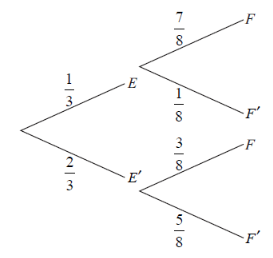
\includegraphics[scale=0.7]{arbre_e_f}\par  
  \medskip
  (a) Trouvez\par
  \hspace{2em}(i)  $P(E \cap F)$\par  
  \hspace{2em}(ii) $P(F)$\hspace*{\fill} [4]\par  
  \medskip
  (b) Trouvez la probabilité que\par
  \hspace{2em}(i)  José rate son bus et ne soit pas en retard à l’école ;\par
  \hspace{2em}(ii) José ait raté son bus, sachant qu’il est en retard à l’école.\hspace*{\fill} [5]\par
  \medskip

  \noindent Le coût pour chaque jour où José prend le bus est 3 euros.\par
  \noindent José va à l’école lundi et mardi.\par
  \medskip

  (c) Recopiez et complétez ce tableau de la distribution de probabilités.\hspace*{\fill} [3]\par
  \medskip
  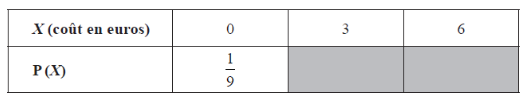
\includegraphics[scale=0.7]{tableau_cout}\par  
  \medskip
  (d) Trouvez l’espérance du coût sur les deux jours pour José.\hspace*{\fill} [2]\par
  
\end{question}

